\section{Caches}

\subsection{Zugriffszeit}
Die Trefferwahrscheinlichkeit für einen Wert in eimem Level-$i$-Cache berechnet siech wie folgt:
\begin{align*}
    P(\text{L1}) &= p_{\text{L1}}                                                                                   \\
    P(\text{L2}) &= p_{\text{L2}} \cdot (\underbracket{1 - P(\text{L1})}_{\text{L1 Miss}})                          \\
    P(\text{L3}) &= p_{\text{L3}} \cdot (\underbracket{1 - P(\text{L1}) - P(\text{L2})}_{\text{L1 und L2 Miss}})    \\
    P(\text{MEM}) &= 1 - (\underbracket{P(\text{L1}) - P(\text{L2}) - P(\text{L3})}_{\text{nicht im Cache}})
\end{align*}
Dabei bezeichnet $p_{\text{L}i}$ den Prozentsatz der Speicher-Lesezugriff, die Cache-Treffer des Level-$i$-
Caches sind. Die mittlere Zugriffszeit auf Werte aus dem Hauptspeicher bzw. dem Cache lässt sich dann wie
folgt berechen:
\[
 T_\avg = P(\text{MEM}) \cdot \left( T_{i - 1} + T_{\text{MEM}} \right) + \sum\left( T_{i} \cdot P(\text{L}_{i}) \right) 
\]
Wobei $T_{i}$ die Zugriffszeit für den Level-$i$-Cache in Nanosekunden ist, $T_{\text{MEM}}$ ist die
Zugriffszeit auf den Hauptspeicher und $T_{i - 1}$ ist der letzte Cache vor dem Hauptspeicher.
\important
$T_{i - 1} \neq 0$, wenn erst \emph{nach} dem letzten Cache auf den Hauptspeicher zugegriffen wird. Bei 
einem parallelen Zugriff auf die Caches und den Hauptspeicher gilt: $T_{i - 1} = 0$.

\subsection{Virtuelle Speicheradresse}

\begin{center}
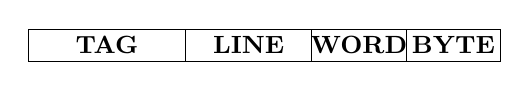
\begin{tikzpicture}[scale=0.4]
\draw (00,00) rectangle (05,01) node[pos=0.5] {\small\textbf{TAG}};
\draw (05,00) rectangle (09,01) node[pos=0.5] {\small\textbf{LINE}};
\draw (09,00) rectangle (12,01) node[pos=0.5] {\small\textbf{WORD}};
\draw (12,00) rectangle (15,01) node[pos=0.5] {\small\textbf{BYTE}};
\end{tikzpicture}
\end{center}

\paragraph{TAG}
Das Feld Tag beshetht aus einem eindeutigen n-Bit-Wert. Er kennzeichnet die entsprechenden
Zeile im Hauptspeicher, woher die Daten stammen. Die Anzahl der Bist wird meist so gewählt
das eine volle Speicheradresse (32/64 Bits) entsteht.
\[
 \text{Bits}_\texttt{TAG} = \text{Bits}_\texttt{ADDRESS} - \text{Bits}_\texttt{LINE} - \text{Bits}_\texttt{WORD}
\]

\paragraph{LINE}
Das Line Feld gibt an, in welcher Zeile sich die entsprechenden Daten befinden, falls diese im Cache
vorhanden sein sollten.
\[
 \text{Bits}_\texttt{LINE} = \left\lceil log_{2}\left(\cfrac{\text{Cachegröße}}{\text{Cachezeilengröße}}\right) \right\rceil
\]

\paragraph{WORD}
Mit dem Word Feld wird angegeben welches Wort aus der Cache Zeile angefordert wird. Dies fällt oftmals
zusammen mit dem \emph{BYTE} Feld, da der Cache lediglich eine Byte-Adressierung zulässt.

\paragraph{BYTE}
Das Byte Feld gibt an welches Byte aus einem Speicherwort geldaen werden soll. Dies kann bei einem Cache
der lediglich eine Byte-Adressierung zulässt auch mit dem \emph{WORD} Feld zusammengefast werden.
\[
 \text{Bits}_\texttt{WORD} = \left\lceil log_{2}\left(\text{Cachezeilengröße}\right) \right\rceil
\]

\subsubsection*{N-Weg-Cache}
Ermöglicht es für eine Speicheradresse mehrere Einträge abzulegen. Dies wird benötig wenn ein Programm
häufig Wörter an zwei weit auseinander liegenden Adressen holt und dadurch ständig Konflikte auftreten 
welche möglicherweße die vorherige Referenz aus dem Cache verdrängt. Ein Zusammfassung $n$ solcher 
Cache-Einträge nennt man \emph{Menge}.
\[
 \text{Anzahl}_\text{Mengen} = \cfrac{\text{Cachegröße}}{\text{Cachezeilengröße} \cdot \text{Assoziativität}}
\]
Da die Kapazität des Caches zunimmt jedoch nicht die Anzahl der adressierbaren Cachezeilen, dadurch muss
die Anzahl der benötigten Bist für die Cachezeilen wiefolgt lauten: 
\[
 \text{Bits}_\texttt{LINE} = \left\lceil log_{2}\left( \text{Anzahl}_\text{Mengen} \right) \right\rceil
\]


\subsection{Schreib-Operationen}
Schreibt der Prozess ein Wort und das Wort befindet sich im Cache, muss der Cache-Eintrag aktualisirt 
werden, heizu gibt es folgende möglichkeiten:
\begin{enumerate}
 \item Cache-Treffer
 \begin{enumerate}
  \item\textbf{Write Through} Die modifizierten Daten werden sofort in den Hauptspeicher zurück geschrieben.
  \item\textbf{Write Back} Die modifizierten Daten werden erst in den Hauptspeicher zurück geschrieben,
  wenn die betroffene Cache-Zeile aus dem Cache entfernt wird.\par (LRU-Algorithmus \emph{Last Recently Used})
 \end{enumerate}

 \item Cache-Verfehlen
 \begin{enumerate}
  \item\textbf{Write Allocation} Erzeugen eines neuen Cache-Eintrags, in den die Daten geschrieben werden.
  \item\textbf{Write Around} Schreiben von Daten direkt in den Hauptspeicher, ohne einen Cache-Eintrag 
  zu erzeugen.
 \end{enumerate}
\end{enumerate}

